\documentclass[border=3pt,tikz]{standalone}
\usepackage{amsmath} % for \text
\usepackage{etoolbox} % ifthen
\usepackage[outline]{contour} % glow around text
\usetikzlibrary{calc} % for adding up coordinates
\usetikzlibrary{decorations.markings,decorations.pathmorphing}
\usetikzlibrary{angles,quotes} % for pic (angle labels)
\usetikzlibrary{arrows.meta} % for arrow size
\usepackage{xfp} % higher precision (16 digits?)
\contourlength{1.1pt}

\tikzset{>=latex} % for LaTeX arrow head
\colorlet{myred}{red!85!black}
\colorlet{myblue}{blue!80!black}
\colorlet{mygreen}{green!80!black}
\colorlet{mydarkred}{red!55!black}
\colorlet{mylightred}{red!85!black!12}
\colorlet{myfieldred}{mydarkred!5} % for S' background
\colorlet{mydarkblue}{blue!50!black}
\colorlet{mylightblue}{blue!50!black!30}
\colorlet{mylightblue2}{myblue!10}
\colorlet{mypurple}{blue!40!red!80!black}
\colorlet{mydarkgreen}{green!50!black}
\colorlet{mydarkpurple}{blue!40!red!50!black}
\colorlet{myorange}{orange!40!yellow!95!black}
\colorlet{mydarkorange}{orange!40!yellow!85!black}
\colorlet{mybrown}{brown!20!orange!90!black}
\colorlet{mydarkbrown}{brown!20!orange!55!black}
\tikzstyle{world line}=[myblue!40,line width=0.3]
\tikzstyle{world line t}=[mypurple!50!myblue!40,line width=0.3]
\tikzstyle{world line'}=[mydarkred!40,line width=0.3]
\tikzstyle{mysmallarr}=[-{Latex[length=3,width=2]},thin]
\tikzstyle{mydashed}=[dash pattern=on 3 off 3]
\tikzstyle{rod}=[mydarkbrown,draw=mydarkbrown,double=mybrown,double distance=2pt,
                 line width=0.2,line cap=round,shorten >=1pt,shorten <=1pt]
\tikzstyle{vector}=[->,line width=1,line cap=round]
\tikzstyle{vector'}=[vector,shorten >=1.2]
\tikzstyle{particle}=[mygreen,line width=0.9]
\tikzstyle{photon}=[-{Latex[length=5,width=4]},myorange,line width=0.8,decorate,
                    decoration={snake,amplitude=1.0,segment length=5,post length=5}]

\def\tick#1#2{\draw[thick] (#1) ++ (#2:0.06) --++ (#2-180:0.12)}
\def\tickp#1#2{\draw[thick,mydarkred] (#1) ++ (#2:0.06) --++ (#2-180:0.12)}
\def\Nsamples{100} % number samples in plot

\begin{document}
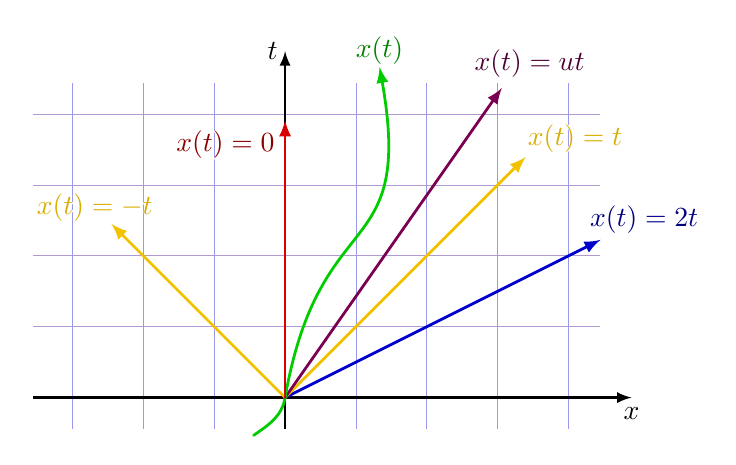
\begin{tikzpicture}[scale=2.0]
  \message{Worldlines^^J}
  
  \def\ymin{0.2}
  \def\xmin{1.6}
  \def\xmax{2}
  \def\Nlines{4} % number of world lines (at constant x/t)
  \pgfmathsetmacro\d{0.9*\xmax/\Nlines} % grid size
  \coordinate (O) at (0,0);
  \coordinate (T) at (0,\xmax+0.2);
  
  % WORLD LINES GRID
  \message{  Making world lines...^^J}
  \foreach \i [evaluate={\x=\i*\d;}] in {1,...,\Nlines}{
    \message{  Running i/N=\i/\Nlines, x=\x...^^J}
    \draw[world line]   ( \x,-\ymin) -- ( \x,\xmax);
    \draw[world line t] (-\xmin, \x) -- (\xmax, \x);
  }
  \draw[world line] (-\d,-\ymin) -- (-\d,\xmax);
  \draw[world line] (-2*\d,-\ymin) -- (-2*\d,\xmax);
  \draw[world line] (-3*\d,-\ymin) -- (-3*\d,\xmax);
  
  % AXES
  \draw[->,thick] (0,-\ymin) -- (T) node[left=-1] {$t$};
  \draw[->,thick] (-\xmin,0) -- (\xmax+0.2,0) node[below=0] {$x$};
  
  % VECTORS
  \draw[vector,myorange] (O) -- (135:0.78*\xmax)
    node[mydarkorange,left=6,above=-3] {\contour{white}{$x(t)=-t$}};
  \draw[vector,myblue] (O) -- ({atan(1/2)}:1.12*\xmax) %(45/2:\xmax)
    node[mydarkblue,anchor=-155,outer sep=-1] {$x(t)=2t$};
  \draw[vector,myorange] (O) -- (45:1.08*\xmax)
    node[mydarkorange,left=1,above right=-2] {\contour{white}{$x(t)=t$}};
  \draw[vector,mypurple] (O) -- (55:1.2*\xmax)
    node[mydarkpurple,right=10,above] {\contour{white}{$x(t)=ut$}};
  \draw[vector,mygreen]
    (-0.10*\xmax,-0.12*\xmax) to[out=35,in=-100] (O)
    to[out=80,in=-80,looseness=1.5] (0.3*\xmax,1.05*\xmax)
    node[mydarkgreen,above=-3] {\contour{white}{$x(t)$}};
  \draw[vector,myred] (O) -- (0,0.88*\xmax)
    node[mydarkred,below left=0] {\contour{white}{$x(t)=0$}};
  %\node[right=8,above,mydarkpurple] at (T) {$x(t)=0$};
  
\end{tikzpicture}
\end{document}